
\chapter{Literature Review\label{ch:pastwork}}

\section{The Impact of Entrepreneurship}

New entrepreneurship is often associated with positive effects on a variety of indicators measuring societal and economic well-being. This ranges from job creation to subsequent economic growth for the region, from sector productivity gains to the invention of new products and industries\footnote{Council on Competitiveness, 2007}\hspace{.15em}\footnote{\cite{Reynolds2007}}. The critical role young firms play in the creation of new sectors is exemplified by the developments associated with products such as smartphones, personal computers, or big box retail outlets\footnote{\cite{GartnerShaverCarterReynolds2004}}. The contributions made by new entrepreneurial activity to job creation in the US economy are hard to overstate - business formation is often associated with the birth of new industries, with innovation and increase in job number and variation\footnote{\cite{ReynoldsWhite1997}}. 

Although policymakers and small business advocates tend to embrace the notion that most new jobs are created by small businesses, empirical research finds that new firms still make for the major source of systematic job expansion in the United States\footnote{\cite{AcsArmington2004}}. Not only is firm age a powerful control under which the effect of firm size decreases in significance\footnote{\cite{HaltiwangerJarminMiranda2013}}, but its contribution to job creation is made evident by simple employment accounting. At the US level, we note a net loss of jobs among businesses aged more than one year, with employment destroyed by ``contractions and terminations'' surpassing the one created by expansions\footnote{\cite{AcsArmington2004}}. As a result, a ``steady influx'' of new firms generating jobs is vital for total employment not to drop, a findings that highlights the pivotal role of startups and young businesses in U.S. job creation\footnote{\cite{AcsArmington2004}}. This contribution pertains to both gross and net job creation, and describes an ``up or out'' path many young firms inscribe themselves onto\footnote{\cite{AcsArmington2004}}. Because of increased capital and scaling pressures new businesses experience, their early survival is dependent on firm growth and increase in capabilities, making for an environment that calls for job creation as an alternative to failure\footnote{\cite{AcsArmington2004}}. In turns, this leads to steady employment growth for the economy as a whole, a phenomenon documented by researchers and targeted by policymakers.

A more difficult to observe, yet just as important contribution new firms bring to an economy such as the U.S. is the associated growth and regional development that tends to follow business creation in the long term. Although endogeneity makes the causal relation between firm formation and economic growth difficult to model, there is an undeniable correlation between the two. This could be telling of both a tendency for rapidly-growing areas to encourage startup formation, as well as the positive effect of young firms on local growth\footnote{\cite{ChatterjiGlaeserKerr2014}}. What research finds is growing evidence that regions with higher levels of firm creation will have greater economic growth in subsequent periods\footnote{\cite{GartnerShaverCarterReynolds2004}}\hspace{.2em}\footnote{\cite{AcsArmington2006}}. 

Glaeser et al. (1992)\footnote{\cite{GlaeserKallalScheinkmanShleifer1992}} observe a strong correlation between small firms and subsequent growth, one that holds true for different measures of entrepreneurship. In Kerr (2010)\footnote{\cite{Kerr2010}} we learn that the geographic location of new patents determines where subsequent ones will occur, indicating an upward trend in patent creation for the given region that can last as long as 30 years from the initial moment. Adding to this, Agrawal et al. (2012)\footnote{\cite{AgrawalCockburnGalassoOettl2012}} denote that a mix of large and small, new firms provides the best regional environment for subsequent innovation. While existing research is far from reaching a consensus regarding the measurable benefits of new firms in regions across the US, it nonetheless indicates there is great power to small startups. This pattern can be extended for countries as well, with higher levels of new firm creation at the national level corresponding to increased levels of economic prosperity\footnote{\cite{GartnerShaverCarterReynolds2004}}. From an economic standpoint, this calls for a better understanding of entrepreneurial decisions as a vital tool for informing policy action. 

\section{Definitions and Measures}

\subsection{Entrepreneurship}

The difficulty of constructing a viable empirical model for the determinants of entrepreneurship stems from the perceived nebulosity of the concept itself. In that sense, economic literature focuses on two distinct approaches to defining entrepreneurship, one invoking the creation of new firms and economic activity and the other, ``the active pursuit of innovation''\footnote{\cite[Page~367]{rocha2004entrepreneurship}}. This is an important distinction, as high-growth entrepreneurship penetrates both policy discussions and the popular imagination, but might not be consistent with firm birth indicators at the U.S. levels. 

The current paper focuses on the first understanding of the concept, capturing new economic activity by individuals regardless of firm size, survival patterns and subsequent impact. This approach is motivated by existing research that testifies to the impact of new businesses in net job creation at the US level\footnote{\cite{HaltiwangerJarminMiranda2013}}. With most U.S. job creation being attributed to new firms, and this serving as a control that moderates the positive effect of small businesses, the need to understand the individual-level decisions that lead to the creation of new companies is a key precursor to better-focused policies meant to spur growth.

\subsection{Necessity vs. Opportunity}

Another important distinction is between entrepreneurship of necessity and that of opportunity. If entrepreneurial activity is preceded by a period of employment at a private or public entity, we refer to it as opportunity entrepreneurship, indicating a change that exploits gained productivity and builds on professional momentum\footnote{\cite{Deli2011}}. If, on the other hand, business formation follows unemployment status, then one is said to be pursuing necessity entrepreneurship, often caused by the lack of labor market adaptation\footnote{\cite{Deli2011}}. Conceptually, this is also viewed as a low-ability/high ability distinction, with entry to self-employment being caused by adverse circumstances in one case, or by a promising idea in the other\footnote{\cite{Deli2011}}. While the two are different in nature, there is a case to be made for each at the policy level, with innovation policy being directed at disruptive technologies and services, or funding made available for people to jumpstart business and drive down unemployment rates. 

The distinction imposed by the activity that precedes entrepreneurship also serves to inform our understanding that not all businesses might be entrepreneurial, or that entrepreneurial behavior can arise independent of firm ownership. In terms of outcomes, when Block and Koellinger (2009)\footnote{\cite{BlockKoellinger2009}} explore the factors associated with self-employment satisfaction, they find that necessity entrepreneurs, the group who became self-employment in lack of better alternative are the least satisfied with their status, in spite of financial controls. In that sense, the process leading to entrepreneurship decisions is said to have an impact on how outcomes unfold, as well as how they are being perceived\footnote{\cite{BlockKoellinger2009}}.

\subsection{Self-Employment}

In applied work, a commonly used proxy for entrepreneurship is self-employment status, designating an individual's work consisting of 15 hours or more on a privately owned business entity\footnote{\cite{BlanchflowerOswald1998}}. Many labor economists denote self-employment as ``the simplest kind of entrepreneurship'', and one of the most comprehensive measures of entrepreneurial activity captured by existing data sources\footnote{\cite{Parker2004}}. Debates still exist, with some authors claiming that ``the self-employed fulfill the entrepreneurial function of being risk-bearing residual claimants''\footnote{\cite[Page 5]{Parker2004}}, while others argue that ``only business owners who co-ordinate factors of production (in particular, those who employ workers) are really entrepreneurs''\footnote{\cite[Page 5]{Parker2004}}.

\subsection{Entrepreneurial Intent}

Adding to the vast literature that focuses on self-employment status as a manifestation of entrepreneurial intent, there is great popular appeal and degree of inevitability to this activity. According to Reynolds and White (1997)\footnote{\cite{ReynoldsWhite1997}}, around two-fifths of the American workforce will have had at least one period of self-employment throughout the course of their lives, with Parker and Ebrary (2004) extending this statistic to two-thirds of people in the U.S. labor force having some form of linkage to self-employment. The survey of literature on entrepreneurship illustrates specific labor patterns associated with this choice, often characterized by independence, self-sufficiency and flexibility at the workplace\footnote{\cite{RodrguezFierroGarridoNavarro2015}}\hspace{.15em}\footnote{\cite{Parker2004}}\hspace{.15em}\footnote{\cite{Quinn1980}}. 

This makes self-employment a valid measure for our purposes, one that captures entrepreneurial spirit as the sustained labor for one's company. As a convention, in what follows we refer to entrepreneurship conceptually, but measure it empirically as self-employment status. Survey evidence indicates that in OECD countries, many current employees would prefer switching to self-employed status\footnote{\cite{BlanchflowerOswald1998}}. Even when taken with a grain of salt, this evidence suggests that there might be restrictions on the supply of entrepreneurs, which makes the study of its determinants an important empirical task to be addressed by the current paper. 


\section{Determinants of Entrepreneurship}

The factors influencing an agent's decision to start a business pertain to both individual-level motivations, as well as environment variables that can facilitate or hinder this action. At the individual level, labor economists focus their research on factors like liquidity, education and marital status, as well as demographic controls such as gender, race and immigration status. The first set of variables denotes individual characteristics that encourage entrepreneurial decisions, while the other, traits that can potentially hinder subjects from entry or success in running their own business. Environment variables concern location, policy incentives, as well as the state of the economy and political climate. 


Despite \textbf{\textit{gender}} being one of the most significant factors in the model for entrepreneurship decisions, little research is dedicated to capturing how self-employment determinants might have differential effects for men and women\footnote{The author of the current paper does not subscribe to the idea of a gender binary. However, given the limitations of current data sources in capturing more than two gender identities, most research focuses on the two categories invoked.}. It is often suggested that agents with diverse characteristics also have ``different objectives and motivations that drive the decision to set up shop''\footnote{\cite{LeoniFalk2010}}, leading to individual-specific approaches to entrepreneurship that policy must account for. In looking at cross-sectional data from Austria's population census, Leoni and Falk (2010)\footnote{\cite{LeoniFalk2010}} find gender differences with respect to SE\footnote{ We introduce SE as an abbreviation for self-employment.}, with women choosing this option less than men. Additionally, when studying patterns in the German labor market, Georgellis and Wall (2005)\footnote{\cite{GeorgellisWall2005}} observe that women seem to treat self-employment as a substitute for inactivity or part-time work to a greater extent. 

A possible explanation accounting for these disparities is an agent's field of study and the persistence of cultural norms and gender-specific occupational strategies\footnote{\cite{CowlingTaylor2001}}. In that respect, authors find that age and field of study factor into the observed gender gap in self-employment, with women underrepresented in science and technology fields at the same level of educational attainment\footnote{\cite{GeorgellisWall2005}}. As industry and skill level play an important part in labor market decisions, gender is closely related to a multitude of asymmetries that might influence entrepreneurial decisions. 

Even though female-owned businesses remain a small portion of male-owned enterprises, SE rates for women in the U.S. have been on the rise over the past decades, as seen in Figure 2.1. 

\begin{figure}[hbtp]
	  \centering{%
		  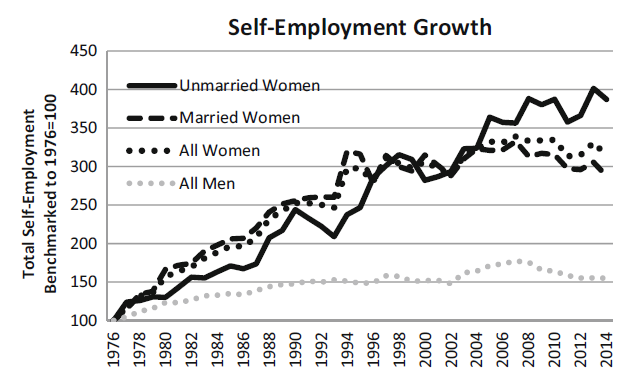
\includegraphics[width=0.75\linewidth]{ch-pastwork/se_growth.PNG}%
    	}%
    \caption{SE Trends in the U.S. Economy (Source: Patrick et al., 2016)} 
\end{figure}

At the U.S. level, recent research advances the idea of different motivations for men and women, with ``more progressive gender attitudes pulling married women from self-employment, while household burdens associated with children pushing them into self-employment as an alternative to not working at all''\footnote{\cite{PatrickStephensWeinstein2016}}. This theory of self-employment as an activity providing married women more resources to balance family and career does not find support in empirical research\footnote{[Wellington, 2006] finds little support that women are increasingly turning to self-employment to balance family and career.}, or the steadily growing share of unmarried women owning a business, observed in Figure 2.1.

\textbf{\textit{Marital status}} is thought to nevertheless affect individual motivations, eliciting different responses to controls. When studies look at data in the aggregate, self-employment is close-to-unanimously positively associated with marital status\footnote{\cite[Page~74]{Parker2004}}. Holding for both business entry and self-employment status, this finding is only weaker in the case of black Americans\footnote{\cite{borjas1986self}} and the English ethnic minority\footnote{\cite{clark2000pushed}}. The general mechanisms thought to explain the positive effect have to do with access to more startup capital in the case of married couples, as well as the availability of labor at below-market rates from the spouse once a business is established\footnote{\cite[Page~75]{Parker2004}}. On top of that, there are associated tax advantages and benefits for the married (healthcare, pension scheme), which can affect the decision to co-enter entrepreneurship\footnote{\cite[Page~75]{BlanchflowerOswald1998}}.

\textbf{\textit{Age}} is often regarded as a proxy for creativity and innovative spirit, one claim being that the older an individual, the less likely to become an entrepreneur. When analyzed in the aggregate, changes in a region's age distribution affect its expected number of startups, the older the population, the lower the share of new businesses\footnote{\cite{Bonte2007}}. In terms of individual patterns, however, the expectation is for most entrepreneurs to be in their 30s and 40s\footnote{\cite{LiangWangLazear2014}}. Work by Quinn (1980)\footnote{\cite{Quinn1980}} tracks labor force participation for older self-employed workers, with results indicating a lower probability to open a business, but also greater chance of maintaining it open. Although most studies address how a region's age distribution influences entrepreneurship rates, or uses an agent's age as a control when testing for other factors, there is growing interest in assessing whether creativity can really be measured via this instrument, and with what results.

The channels through which \textbf{\textit{education}} factors into self-employment are also of great interest to researchers, studies tracking its effect on entry decisions, outcomes, as well as the many other aspects pertaining to running one's business. Higher education and business knowledge are seen as preconditions for ``opening up shop'', yet the expected sign of this coefficient on the probability of becoming self-employed is to be debated. Some authors suggest higher education is a decisive determinant of initial entry into SE, with highly skilled individuals having a higher self-employment rate than other groups in the labor force\footnote{\cite{rees1986empirical}}\hspace{.15em} \footnote{\cite{robinson1994effect}}\hspace{.15em} \footnote{\cite{luber2000growing}}. Yet, when separating boom and bust periods in Finland, Kangasharju and Pekkala (2001)\footnote{\cite{kangasharju2001regional}} find an opposing pattern, with the highly educated being less likely to become self-employed in periods of economic upturn. This finding can be explained by the higher outside demand highly-educated agents experience for their labor, as well as the utility tradeoff associated with entrepreneurship in their case\footnote{\cite{kangasharju2001regional}}. In that sense, running a small firm might not be as attractive as wage work due to ``lower earnings prospects, less stable stream of earnings and the cultural tradition of working in large corporations''\footnote{\cite{kangasharju2001regional}}. In terms of exit rates, the highly educated are also found to have higher exit probability in times of boom, for demand-side reasons similar to those invoked before\footnote{\cite{kangasharju2001regional}}.

Moving beyond years of education and into a discussion of skills more broadly, Lazear (2005)\footnote{\cite{Lazear2005}} introduced the hypothesis that more versatile individuals have higher entrepreneurship rates, with \textbf{\textit{diversified skills}} mattering more than specialized expertise. This has many implications, one being that versatile education, a trait rather difficult to measure with available data, might matter more than higher education in econometric models of entrepreneurship. In terms of entry determinants, versatility as invoked by the author could also be instrumented by a change in industry, if observed to have a significant effect on entrepreneurship decisions. Under this assumption, if entrepreneurial activity is found to be associated with a change in industry, then there's a high degree of adaptability to an individual's skills. The versatility assumption would then paint the picture of entrepreneurs as ``jacks of all trades'' (in Lazear's terminology), able to switch from an industry to the other when starting their own business.

\textbf{\textit{Race}} is an important control for self-employment entry and success patterns, as it speaks to persistent disparities in U.S. business ownership\footnote{ More than 10\% of US workers are self-employed business owners, holding 37.4 percent of total U.S. wealth, yet only 5.1 percent of African American workers and 7.5 percent of Latino workers own businesses compared with more than 11 percent of white and Asian workers (Fairlie and Robb, 2008).}. Having roots in existing racial inequality in education, income, or wealth at the U.S. level, these differences are less understood, with major implications for productivity and economic growth\footnote{\cite{ReynoldsWhite1997}}. The most recent findings place African Americans and Latinos at a lower likelihood to own a business than whites and Asian Americans, and more likely to underperform in running it (lower sales and profits, fewer employees and high closure rates)\footnote{\cite{FairlieRobb2008}}. These patterns speak to the effects of existing disparities, with black-owned businesses starting with substantially less financial capital, and having owners with lower levels of education and business experience on average\footnote{\cite{FairlieRobb2008}}. This extends to exit rates, with higher probabilities to ``close shop'' for Latinos and African Americans\footnote{\cite{FairlieRobb2008}}. At the opposite end, Asian American firms have the strongest performance among racial and ethnic groups after controlling for firm size\footnote{\cite{FairlieRobb2008}}. At the same time, they are more likely to have college educated-owners, an artefact of education patterns at the U.S. level\footnote{\cite{FairlieRobb2008}}.

\textbf{\textit{Immigration status}} is an individual-level variable of key significance, with two opposing views described in literature for its effects on the U.S. economy.
\renewcommand{\labelenumi}{\roman{enumi}}
\begin{enumerate}
  \item Classical economic theory predicts an increases in immigration should decrease employment and price of labor for the native workforce, as it decreases the labor market competitiveness of the later\footnote{\cite{Hanson2012}}. 
  \item Other authors argue that historically, improvements in American living standards have been the consequence of productivity growth, both of capital and labor, a growth resulted from the many innovations in which immigrants often played a key role\footnote{\cite{jones1995culture}}
\end{enumerate}
The body of research on immigration status was incapable of substantiating the belief stemming from classical theory. In turn, high-skilled immigrants are said to make for a growing 25\% of U.S. entrepreneurs, and have equal, if not higher contributions to the production of patents and economic output than natives\footnote{\cite{Kerr2013}}. On average, immigrants also seem to be better trained than natives, when skills are conditioned on educational attainment of comparable levels\footnote{\cite{Kerr2013}}. Although findings attest for the contributions of highly-skilled immigrant entrepreneurs to the U.S. economy, immigration continues to be a divisive issue at the U.S. level, with few, often-blocked policy responses to the consensus in empirical findings\footnote{\cite{Hanson2012}}. 

\textbf{\textit{Availability of capital}} is thought to be a key factor in entrepreneurship decisions, acting as an impediment when not satisfied, as well as an encouraging factor when in abundance. Works by Evans and Leighton (1989)\footnote{\cite{EvansLeighton1989}} or Evans and Jovanovic (1989)\footnote{\cite{EvansJovanovic1989}} find that ceteris paribus, people with greater family assets have a higher probability of switching into self-employment from wage employment. Adding to this, more recent research from Dunn & Holtz-Eakin (2000)\footnote{\cite{DunnHoltzEakin2000}} or Georgellis and Wall (2005)\footnote{\cite{GeorgellisWall2005}} reveals that unexpected gains, such as inheritance or redundancy payments, increase the probability of switching to self-employment. At the other end of the spectrum, capital constraints are the most invoked difficulty by potential entrepreneurs when surveyed about business entry\footnote{\cite{BlanchflowerOswald1998}}. Looking at individual characteristics tracked as far back as childhood personality measurements, Blanchflower and Oswald (1998)\footnote{\cite{BlanchflowerOswald1998}} find no predicting power, and conclude that access to start-up capital remains what matters most for entry decisions. Adding to the access-to-capital framework, Fairlie and Robb (2008)\footnote{\cite{FairlieRobb2008}} find a ``strong positive relationship between startup capital and business outcomes'', firms with higher liquidity levels upon startup being more likely to survive and earn more profit in the long term.

Entrepreneurial activity cannot exist in a vacuum, and often times, business owners are dependent on their partners, on existing social networks and professional ties\footnote{\cite{Lerner2009}}\hspace{.15em}\footnote{\cite[Page~74]{Parker2004}}. \textbf{\textit{Social capital}} matters for business formation, along with existing norms that might inform one's expectations of success\footnote{\cite{Lerner2009}}. Yet, research has been slow to quantify the effects of social capital on entrepreneurship decisions, with most work adopting a sociological perspective of the co-owned business startup. \textit{The Entrepreneurial Group} cites recent surveys denoting that more than half of American business owners hold shared ownership of their startups, going against portrayals of ``the lone visionary'' entrepreneur\footnote{\cite{Ruef2010}}. According to the authors, groups have positive effects on securing credit and advancing initiatives, contributing to higher entry rates\footnote{\cite{Ruef2010}}. Fairlie and Robb (2008)\footnote{\cite{FairlieRobb2008}} complement these findings, denoting that more business experience within a founder's family leads to better outcomes for the enterprise and thus, lower exit probability\footnote{\cite{FairlieRobb2008}}. 


Although some authors claim that urban economics has failed to deliver sufficient work on the spatial aspects of entrepreneurship\footnote{\cite{GlaeserRosenthalStrange2009}}, existing research points to the importance of the \textbf{\textit{local environment}} in the choices of entrepreneurs, as well as subsequent success and influence on the local economy. Self-employment rates vary at the U.S level, with the local business climate and entrepreneurial culture of a region acting as a deterrent or a draw\footnote{\cite{PatrickStephensWeinstein2016}}. Location is often studied in parallel with industry, affecting entrepreneurship decisions via proximity to necessary resources or adherence to economic clusters. One key factor is the concentration of funding sources, the easiest to name being VC investments, with 50\% of total funding going to Silicon Valley and Boston, when these regions only hold 11\% of US population\footnote{\cite{ChatterjiGlaeserKerr2014}}. 

When studying the local determinants of manufacturing startups across cities and industries, Glaeser and Kerr (2008)\footnote{\cite{GlaeserKerr2008}} find that entry is predicted by the presence of local customers, and that new entrants are often drawn to areas with many small suppliers. Ghani et al. (2011)\footnote{\cite{GhaniKerrOConnell2011}} find that the higher the female ownership of local businesses in related industries, the greater the entry rate for new female entrepreneurs, leading to regional spillover effects\footnote{\cite{GhaniKerrOConnell2011}}. This points to the existence of a local entrepreneurship culture, sensible to industry effects and existing gender norms. Adding to this, location variables can also control for uneven natural advantages, or geographic clustering caused by other types of forces, such as the desire to live in NYC, or the location of top research universities\footnote{\cite{ChatterjiGlaeserKerr2014}}. 

\textit{\textbf{Industries}} have evolved, organically or not, to be fairly concentrated in the U.S., attracting business formation via existing opportunities, but also hindering it through persistent entry barriers for particular groups\footnote{\cite{ChatterjiGlaeserKerr2014}}. On the one hand, there are fields that receive significant attention for their innovative characteristics, and that welcome new businesses every year, a prominent example being offered by the tech industry and its growth over the past two decades\footnote{\cite{Berman2014}}. On the other hand, however,  industry segregation by skill level, gender or minority status is still prominent, with a clear lack of diversity across many NAICS subcategories\footnote{\cite{cartwright2011job}}. 

Half a century after the Equal Pay Act of 1963 was passed, women are still found to earn less than men across the board, with industry-specific effects perpetuating these steady trends\footnote{\cite{corbett2012graduating}}\hspace{.15em}\footnote{\cite{cartwright2011job}}. In terms of self-employment participation, the ``disadvantaged worker theory'' denotes that factors hindering general labor market participation might, in fact, encourage workers to start their own business\footnote{\cite{PatrickStephensWeinstein2016}}. The entrepreneurial process would then be seen as both a way to break barriers, as well as an intermediary step toward wage employment\footnote{\cite{PatrickStephensWeinstein2016}}. This theory has nonetheless not echoed in many empirical applications, the convention in literature being to use industry-fixed effects when modeling self-employment status.

The local and national \textbf{\textit{policy environment}} can affect individual entrepreneurship decisions via multiple channels, from helping address liquidity constraints to imposing extra restrictions, from changing corporate taxes to being responsible for the institutional quality and the degree of economic freedom in a given region\footnote{\cite{Williams2013}}. While government loan programs have been found to be generally ineffective in spurring entrepreneurship rates, taxes can have a pronounced effect on the local business climate, being one of the most comprehensively studied factors of innovation policy\footnote{Works include \cite{CullenGordon2006}; \cite{DjankovGanserMcLieshRamalhoShleifer2008}; \cite{Goetz2008}; \cite{Lerner2009}; \cite{Williams2013}.}. To this regard, Djankov et al. (2008)\footnote{\cite{DjankovGanserMcLieshRamalhoShleifer2008}} find that a 10\% increase in the effective corporate tax rate\footnote{ This rate is obtained by dividing a company's total tax bill by its profits.} reduces aggregate investment to GDP ratio by 2 percentage points, and has an adverse impact on entrepreneurial activity. 

Cullen and Gordon (2002)\footnote{\cite{CullenGordon2002}} look at individual incentives, showing that taxes affect the decision to become an entrepreneur due to differences in tax rates on business vs. wage income, as well as the asymmetric tax treatment of losses vs. profits. Using individual tax returns at the U.S. level, their findings reveal that tax law can significantly alter behavior and distort the decision to start a business\footnote{\cite{CullenGordon2002}}. More difficult to measure, institutional quality and the degree of economic freedom also factor into entry and exit decisions, with attempts to quantify the magnitude of their positive effects on self-employment rate\footnote{\cite{Williams2013}}.

Our review of educational attainment and its effects noted that potential founders respond differently to the \textbf{\textit{economic climate}} based on their level of education. In that sense, measures of local economic upturn/downturn affect the opportunity cost of individuals upon switching to self-employment, as well as the expected utility from this activity. Periods of economic boom have negative effects on SE rates for highly-skilled workers, with wage-employment being more advantageous and in greater supply\footnote{\cite{kangasharju2001regional}}. 

In line with the opportunity/necessity distinction in entrepreneurship motivations, \textbf{\textit{unemployment}} can have a positive effect on entry SE rates, with individuals starting a business as an alternative to remaining unemployed\footnote{\cite{Deli2011}}. Research confirms this pattern, finding a positive correlation between local unemployment rates and entry into self-employment for low-ability workers\footnote{\cite{Deli2011}}. These results however, do not hold for high-ability workers, for which there is a negative correlation between unemployment and self-employment\footnote{\cite{Deli2011}}. The interaction between ability and unemployment status is a key component for this type of analysis, speaking to the opportunity cost of highly-skilled workers joining self-employment. 













